\chapter{The New PerLa Middleware}
\label{cha:middleware_overview}

\section{Design goals}

Introduce the design goals of the new Middleware architecture

\section{Overview of the New Middleware Architecture}

As illustrated in the previous chapter, the PerLa Middleware is responsible for
managing the lifecycle of all devices connected to the PerLa System, and for
providing a uniform API to interact with them. Its design revolves around the
Functionality Proxy Component (\texttt{FPC}), a self-contained proxy object
that embeds all the logic required to communicate with a single remote device.
The most prominent trait of the \texttt{FPC} is its interface, an API that
allows PerLa users to interact with the sensing network through a compact set
of hardware-agnostic communication primitives reminiscent of classic Java
getter and setter methods. Use of this interface neither requires knowledge of
the sensing network, nor of the device that will ultimately perform the
requested operation.

\begin{figure}[h!]
\includegraphics[width=\textwidth]{imgs/middleware_overview.pdf}
\caption{The New PerLa Middleware architecture}
\end{figure}

\subsection{The New FPC}

Differently from the Classic PerLa Middleware, the New \texttt{FPC} is formed
from the composition of various independent software units, each of which is
responsible for the management of a single aspect of the interaction with the
remote device (see figure~\ref{fig:fpc_overview}). This new modular design was
chosen to further promote reusability and foster future expandability through
composition of independent objects. The remainder of this section contains a
summary of all modules that compose the new \texttt{FPC} architecture.

\begin{figure}[h!]
\center
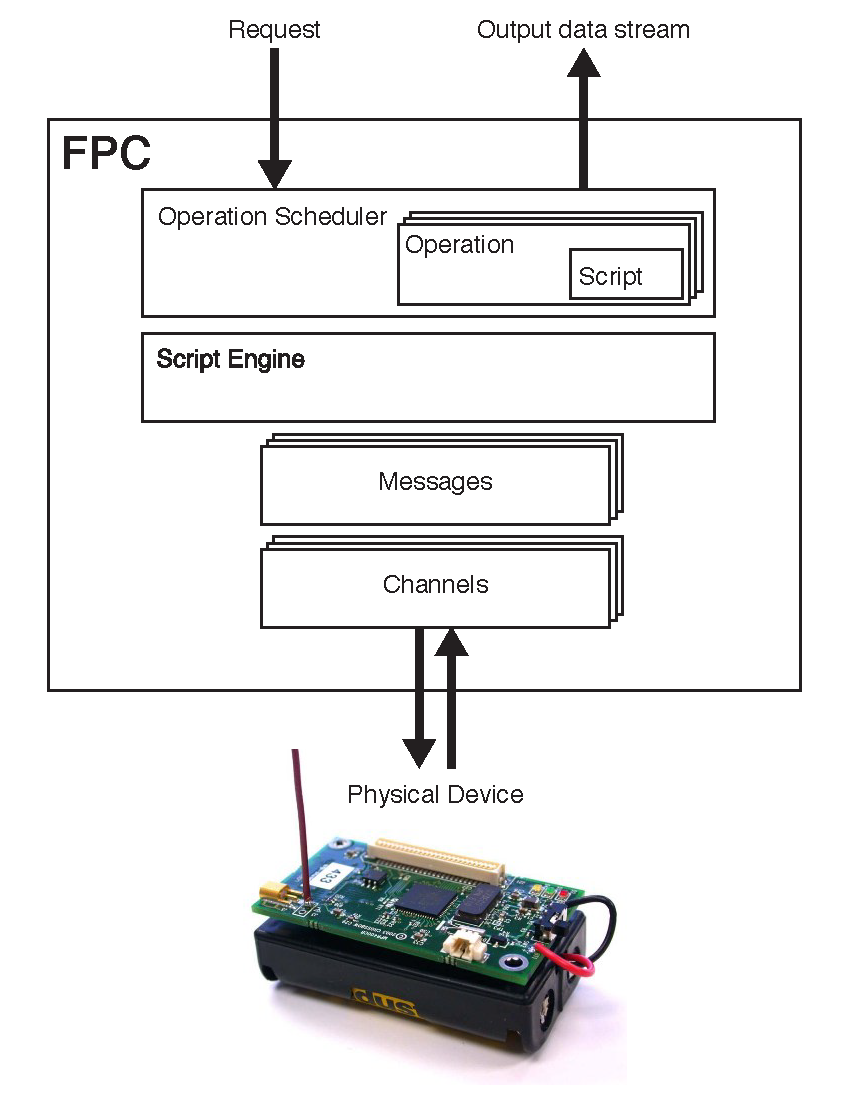
\includegraphics[width=0.6\textwidth]{imgs/fpc.pdf}
\caption{Internal structure of the New FPC.}
\label{fig:fpc_overview}
\end{figure}

\subsubsection{Channel}

\texttt{Channel}s are software components capable of performing I/O operations.
They are commonly employed to manage the communication between PerLa and the
devices of a Pervasive System, and can be thought as a complete substitute of
the \texttt{Channel Manager}/\texttt{Virtual Channel} component pair. Unlike
their counterpart in the Classic architecture, \texttt{Channel}s are settled
inside the boundary of an \texttt{FPC}. This change of location has two
important consequences: first of all, it allows each \texttt{FPC} to make use
of multiple data transmission technologies for the exchange of information with
the controlled endpoint; second, it enhances the modularity of the entire PerLa
Middleware, as new communication systems and protocols can be introduced
without modifying any existing \texttt{Channel} implementations.

Every \texttt{Channel} is bundled with a collection of \texttt{IORequest}
objects, which are employed to initiate specific I/O tasks on the sensing
nodes. For example, the \texttt{HTTPChannel} --- a \texttt{Channel}
implementation of the HTTP protocol --- is bundled with four different
\texttt{IORequest}s, one for each of the principal HTTP methods (GET, POST, PUT
and DELETE).

\subsubsection{Mapper}

A software module for marshalling and unmarshalling data. \texttt{Mapper}s
allow the \texttt{FPC} to interpret byte streams received from a communication
\texttt{Channel}, and to serialize high-level data structures prior to
transmission. They perform as a more flexible alternative to the fixed
\texttt{Marshaller}-\texttt{Unmarshaller} components found in the Classic
\texttt{FPC} implementation.

Every \texttt{Mapper} is a discrete component responsible for managing a
specific \texttt{Message} format. Therefore, similarly to what already seen for
the \texttt{Channel}, a single \texttt{FPC} may employ different
\texttt{Mapper} objects tasked with managing a well-defined set of data
structures exchanged with the remote device. This feature is in stark contrast
with the Classic Middleware design, which could only handle a single data
format per device.

\subsubsection{Scripts and Operations}

\texttt{Script}s and \texttt{Operation}s are a new addition to the PerLa
Middleware. Their primary duty consists in binding high-level data requests to
native processing tasks performed on the remote device.

\texttt{Script}s are interpreted programs written using the \textit{PerLa
scripting language}, a simple imperative programming language designed for
interacting with sensing nodes, and for mapping the contents of a low-level
data structure to the high-level \texttt{Attribute}s generated by an
\texttt{FPC}. \texttt{Scrip}s are executed by a singleton component denominated
\texttt{Script Engine}.

\texttt{Operation}s, on the other hand, are data management entities that
incorporate one or more \texttt{Script}s dedicated to a specific purpose. The
New Middleware architecture distinguishes between four \texttt{Operation}
types, corresponding to different data collection or transmission strategies:

\begin{itemize}

    \item \texttt{Get Operation:} retrieves a single sample from the remote
        device;

    \item \texttt{Set Operation:} transmits data to the remote device;

    \item \texttt{Periodic Operation:} manages the periodic collection of data
        samples generated by an endpoint of the Pervasive Network;

    \item \texttt{Async Operation:} handles the reception of asynchronous
        events emitted by the controlled node.

\end{itemize}

It is important to note that every \texttt{Operation} is associated with the
set of Device \texttt{Attribute}s that can extract or set through it.
Therefore, under the New Middleware architecture, a typical data collection
request is executed as follows:

\begin{enumerate}

    \item The \texttt{FPC} selects an \texttt{Operation} that can be used to
        adequately retrieve the \texttt{Attribute}s requested by the user;

    \item The \texttt{Operation}'s initialization \texttt{Script}s, if any, are
        executed in order to configure the remote device and commence the
        collection of data;

    \item Every data sample received from the \texttt{FPC} is processed by a
        \texttt{Script}, as per \texttt{Operation} instructions, which is
        tasked with unmarshalling the information sent by the endpoint and
        create a new output record.

\end{enumerate}

\section{FPCFactory}
\label{sec:newmiddleware.factory}

The new \texttt{FPCFactory} is a modular software entity composed of multiple
factory components dedicated to the creation of a specific \texttt{FPC} module.
Its design is a significant departure from the original monolithic factory
structure, and allows final users to easily expand the base capabilities of the
PerLa Middleware without modifying its original source code. This modular
architecture, formally called \texttt{FPCFactory} Plugin System, is a direct
implementation of the \textit{Open/Close} principle: the \texttt{FPCFactory} is
open for extension, as its functionalities can be expanded by adding new
plugins, but closed for modification, since the addition of a new sub-factory
modules does not require any change to the Middleware's source code.

At the current state of implementation, the PerLa Middleware supports three
different \texttt{FPCFactory} plugin types, viz. \texttt{ChannelFactories},
\texttt{IORequestFactories} and \texttt{MapperFactories}, which are responsible
for the creation of new \texttt{Channels}, \texttt{IORequests} and
\texttt{Mappers} respectively. All implementations of a single plugin type are
tasked with creating the same class of \texttt{FPC} modules, but are allowed
different behaviours; for example, the \texttt{HTTPChannelFactory} and the
\texttt{TinyOSChannelFactory} both create \texttt{Channel} objects, but the
first are used to connect with RESTful web APIs, whereas the second are
interfaces to TinyOS networks.

The introduction of a new modular \texttt{FPCFactory} Plugin System resulted in
a complete redesign of the Device Descriptor itself, which changed its layout
to accomodate a modular structure that closely follows the new
\texttt{FPCFactory} architecture. The new Device Descriptor is composed of the
following elements:

\begin{itemize}

    \item \textbf{Preamble:} Represented by the root \lstinline!<device>! tag,
        this section contains a textual description of the endpoint, and a list
        of XML namespaces. As shown later, namespaces are employed to select
        the various Device Descriptor features and \texttt{FPCFactory} plugins
        required for the creation of an \texttt{FPC} object;

    \item \textbf{Attribute declarations:} A list of all the
        \texttt{Attributes} exposed by the device. It must be enclosed in an
        \lstinline!<attribute>! XML tag;

    \item \textbf{Channel declarations:} This section contains the
        configuration options of all \texttt{Channel} objects required to
        communicate with the remote device. Its contents are parsed and
        interpreted by the individual \texttt{ChannelFactory} plugins, whose
        structure is discussed in section~\ref{sec:channel};

    \item \textbf{Request declarations:} This part of the Device Descriptor is
        reserved for the declaration of all \texttt{IORequest} objects needed
        to communicate with a remote device. The elements hereby contained are
        processed by the \texttt{IORequestFactory} plugins, as per instructions
        given in section~\ref{sec:channel};

    \item \textbf{Message declarations:} A section reserved for the declaration
        of all data structures required to exchange information with a node of
        the network. Its contents are directly interpreted by the
        \texttt{MapperFactory} plugins to create new \texttt{Message}
        mappers, as described in section~\ref{sec:components.mapper};

    \item \textbf{Operation declarations:} As shown in
        section~\ref{sec:components.fpc}, this final portion of the Device
        Descriptor contains all PerLa \texttt{Scripts} employed to control the
        remote device.

\end{itemize}

~\\
\lstset{language=XML}
\begin{lstlisting}[caption={The skeleton of the new XML Device Descriptor.}]
<?xml version="1.0" encoding="UTF-8"?>
<device type="test" xmlns="http://perla.dei.org/device">
  <attribute>
    <!-- Attribute declarations -->
  </attribute>
  <channel>
    <!-- Channel declarations -->
  </channel>
  <message>
    <!-- Message declarations -->
  </message>
  <request>
    <!-- IORequest declarations -->
  </request>
  <operation>
    <!-- Operation and Scripts -->
  </operation>
</device>
\end{lstlisting}

As briefly explained in previous paragraphs, XML namespaces constitute a
fundamental element of the \texttt{FPCFactory} Plugin System, since they are
used to select which factory component must be employed for the creation of a
specific \texttt{FPC} module. A practical example of this concept is available
in figure~\ref{fig:dd_namespace}: this Device Descriptor excerpt specifies two
plugin namespaces, one for a \texttt{HTTPChannel}
(\texttt{http://perla.dei.org/fpc/channel/http}), and the other for a
\texttt{JSONMapper} (\texttt{http://perla.dei.org/fpc/message/json}); these two
values, once processed by the texttt{FPCFactory}, are used for selecting the
specific plugin that will be used for constructing the corresponding
\texttt{FPC} components. It is important to note that the
\texttt{http://perla.dei.org/device} and
\texttt{http://perla.dei.org/device/instructions} namespaces included in this
example are mandatory, as they respectively define the Device Descriptor base
elements and all available \texttt{Script} instructions.

\begin{figure}[h!]
\center
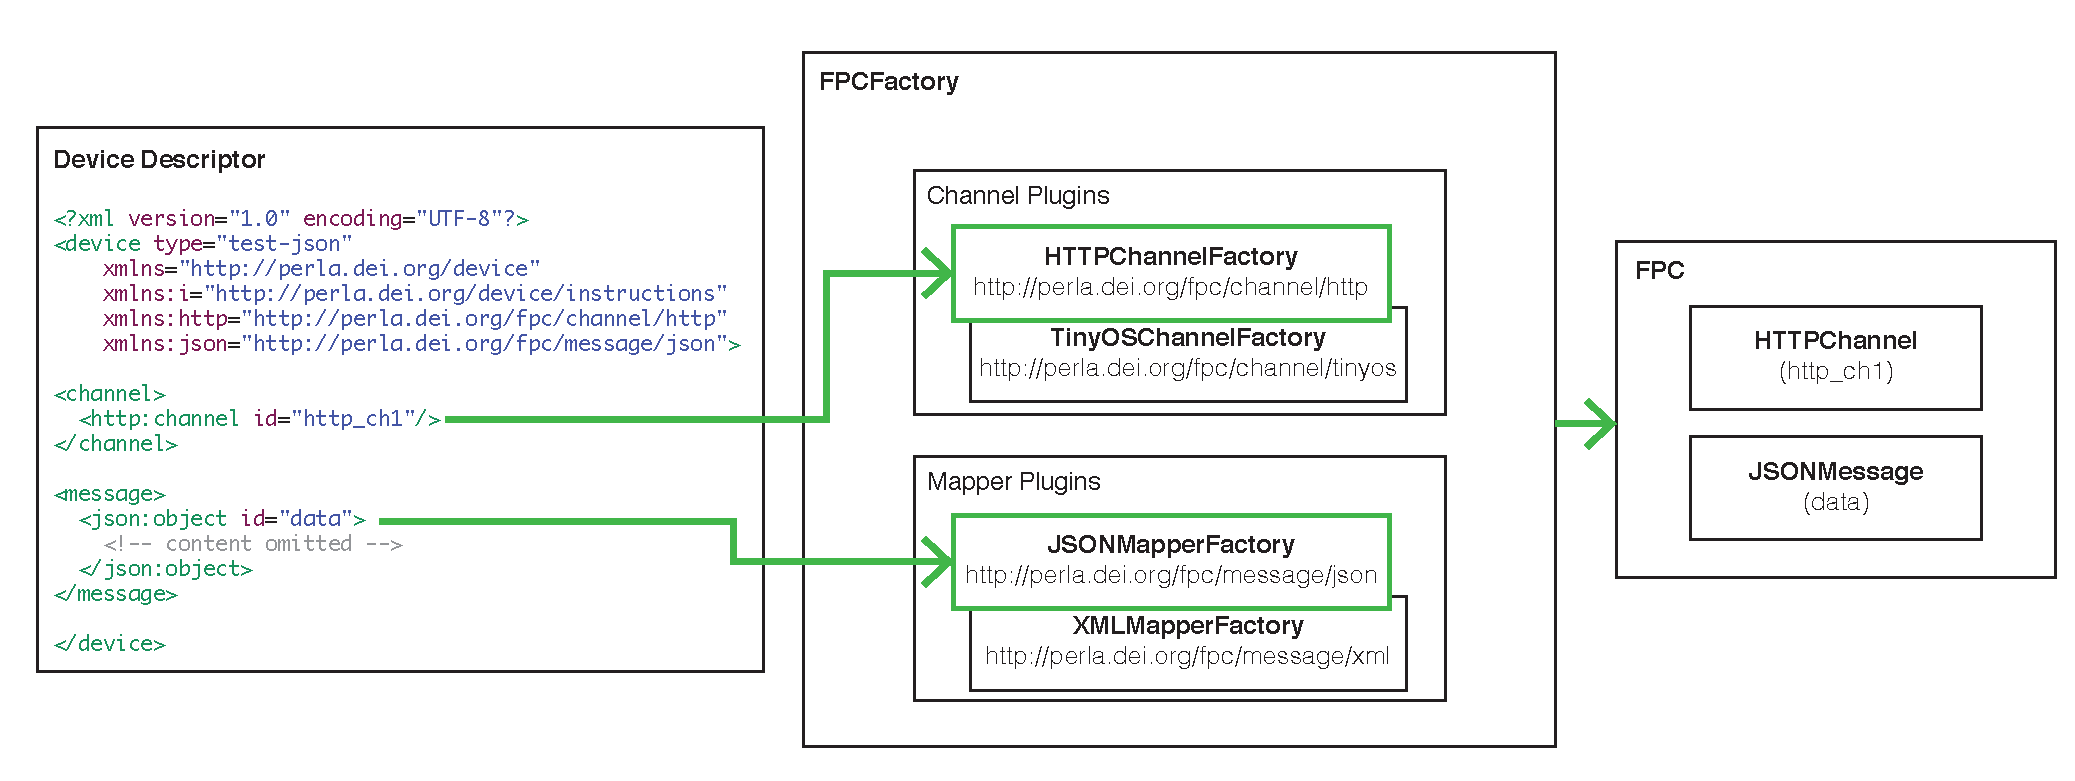
\includegraphics[width=\textwidth]{imgs/dd_namespace.pdf}
\caption{Namespace-guided FPC creation.}
\label{fig:dd_namespace}
\end{figure}

Every \texttt{FPCFactory} plugin is also responsible for defining the
particular XML syntax to be used in its Device Descriptor section. This feature
endows plugin authors with the opportunity to specify a custom set of options
to be used for the creation of their \texttt{FPC} modules. The possibility of
using a custom syntax is key to the new \texttt{FPCFactory} Plugin System,
since different types of plugins may require totally different configuration
values in order to be used or even initialized (e.g., communicating over a HTTP
\texttt{Channel} is considerably different than sending data on a low-power
mesh network).


\section{Asynchronous interaction paradigm}
\label{sec:newmiddleware.async}

The last differences between the New and Classic Middleware architectures lies
in the technique employed to interconnect internal modules of the PerLa
software infrastructure. The New Middleware introduces a fully asynchronous
interaction paradigm based on non-blocking method invocations and event-driven
programming techniques, which deviates profoundly from the mechanism previously
promoted in the Classic design.

\begin{figure}[h!]
    \center
    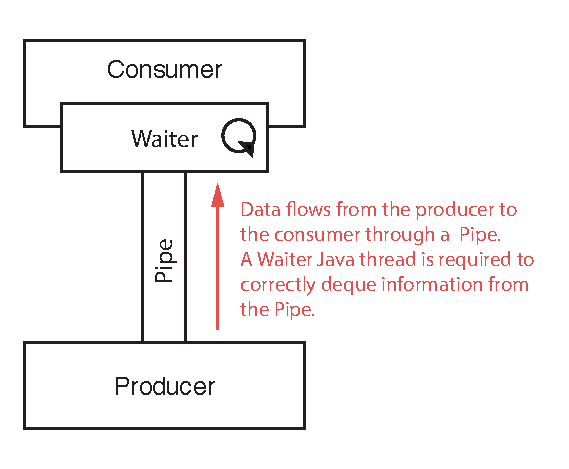
\includegraphics[width=0.5\textwidth]{imgs/pipe_waiter.pdf}
    \caption{A typical \texttt{Pipe}-\texttt{Waiter} connection in the Classic
        PerLa Middleware}
\end{figure}

Within the previous Middleware architecture, a connection between two different
modules was achieved by means of a decoupling element dubbed \texttt{Pipe}, a
one-way message queue designed to shuttle data elements from a software
component to its intended receiver. This system proved to be crucial in the
first development stages of PerLa, as its generic interface allowed the early
designers to experiment with several competing architectures and component
combinations. However, its flexibility came at a cost, both in terms of
performances and API readability. First of all, each \texttt{Pipe} allocated an
initial memory cache of 10 elements. Moreover, the receiving end of a
\texttt{Pipe}, namely the \texttt{Waiter}, was required to instantiate a Java
thread dedicated solely to the reception of data messages. The widespread use
of the \texttt{Pipe}-\texttt{Waiter} paradigm thus led to the proliferation of
threads and to an overuse of memory, which negatively impacted the overall
system efficiency. In addition, the loosely coupled interaction paradigm
promoted by the Classic Middleware resulted in a weak API that lacked intent
and semantic clarity.

The asynchronous, event-driven architecture implemented in the New Middleware
overcomes all aforementioned drawbacks, and improves system performances in
terms of both throughput and scalability. Differently from the deprecated
\texttt{Pipe}-driven system, this new design fosters a direct exchange of
information between data producers and data consumers; information is no more
delivered using a mandatory middleman (i.e., the \texttt{Pipe}), but is
explicitly handed over to the intended recipients. This interaction paradigm is
based on the \textit{Hollywood Principle}, a software design methodology whose
tenets are summarized by the motto ``\textit{don't call us, we call you}'',
that encourages the development of highly-cohesive, low-coupling APIs, 

\begin{figure}[h!]
\center
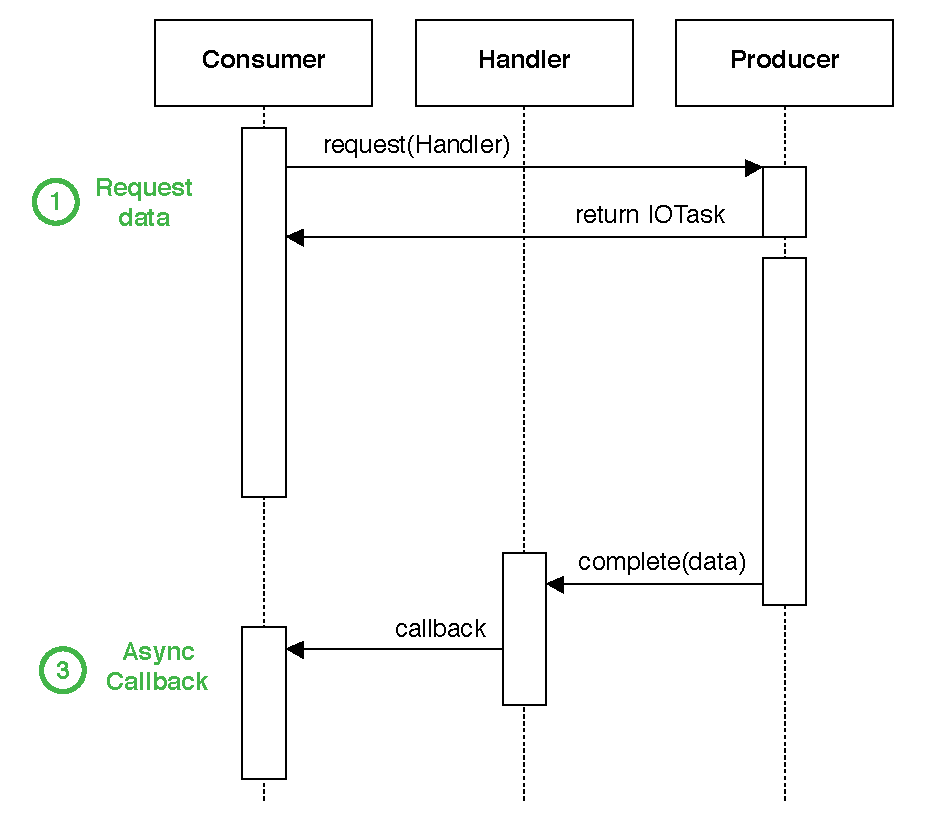
\includegraphics[width=0.8\textwidth]{imgs/async_paradigm.pdf}
\caption{Sequence diagram of an asynchronous method call. Note that the
consumer and the producer continue their execution in parallel.}
\label{fig:async_paradigm}
\end{figure}

Every asynchronous method call in the New PerLa Middleware is identified by the
following characteristics:

\begin{itemize}

    \item \textbf{Does not block:} Calls to an asynchronous method never block;
        control of the execution flow is immediately returned to the caller,
        and the requested computation is executed asynchronously. This
        characteristics reduces the number of Java threads that the caller
        module needs to instantiate;

    \item \textbf{Returns a Task object:} Asynchronous method calls do not
        return the immediate result of a computation. Instead, they return a
        \texttt{Task}, i.e., an object that can be employed to stop the ongoing
        operation or to query its current state of progress;

    \item \textbf{Defers the delivery of results:} The effective result of an
        asynchronous method is notified through a \texttt{Handler} function,
        which is invoked as soon as the computation terminates.

\end{itemize}

For an in-depth description of the actual asynchronous APIs implemented within
the PerLa Middleware, refer to chapter~\ref{cha:components}.

